% https://habr.com/ru/companies/ruvds/articles/574352/
% https://guides.nyu.edu/LaTeX/sample-document

\documentclass{article}
\usepackage[utf8]{inputenc}
\usepackage[english,russian]{babel}

\usepackage{graphicx}

\title{Экономические эффекты автоматизации с ИТ}
\author{А. Е. Моисеев}
\date{февраль 2024}
%\date \today

\graphicspath{ {img/} }

\begin{document}

\maketitle

В переписи населения США 1890-го года перфокартные машины Германа Холлерита позволили обработать 63 млн. анкет за два года\footnote{Population and Area (Historical Censuses) \cite{usCentus}}\footnote{The Punched Card Tabulator, IBM’s 100 Icons of Progress \cite{ibmPuchCard}}. В этот раз впервые была применена новая технология: каждая перфокарта представляла собой анкету участника переписи, представленную в таком специальном виде, в котором с ней могла работать специально сконструированная электромеханическая машина для подсчета статистики. В предыдущей переписи 1880-го года работа велась вручную — меньшее на четверть количество анкет обрабатывали вчетверо дольше — восемь лет. Так начиналась история компании IBM и история массового внедрения технологий автоматической обработки данных. К 1913-му году технологии автоматической обработки данных на базе перфокартных машин уже применялись на фабриках, сталелитейных заводах, страховых компаниях, телефонных компаниях, компаниях оптовой торговли, муниципалитетах, государственных учреждениях и в множестве других сегментов экономики\footnote{The Hollerith tabulating machine in business office \cite{machinery1913}}.

Руководителям Бюро переписи не нужно было объяснять, зачем производить «цифровую трансформацию»: замена ручного труда автоматами дала радикальное повышение производительности труда сотрудников, обрабатывавших анкеты. В условиях значительного притока населения без средств автоматизации они просто не смогли бы завершить обработку результатов грядущей переписи до начала следующей. Кроме сокращения необходимого времени, новые автоматы позволили посчитать гораздо более сложные статистические коэффициенты. В современном мире, когда средства автоматизации работы с информацией в том или ином виде уже используются в организациях, преимущества от внедрения очередного программного пакета или подписки на очередной цифровой сервис может быть не так легко оценить.

Технологии, основанные на цифровых вычислениях, оказались достаточно универсальными для того, чтобы проникнуть во множество сегментов экономики и повседневной жизни. На рынке представлены разнообразные продукты, в том или ином виде включающие цифровую программную составляющую: лицензионное программное обеспечение («чистое» ПО), аппаратно-программные платформы, облачная аппаратно-программная инфраструктура. Для покупателя имеют значение расходы на приобретение и внедрение продукта, а также выгода, которую получает организация от его внедрения, — \textit{экономический эффект}\footnote{«the total effect is reflected in an improved and increased product at a lower cost», H. L. Gantt, Organizing for work, 1919, стр. 91 \cite{ecoEffectOrganizingForWork}} автоматизации. Если выгода от внедрения продукта превышает расходы, то такую покупку имеет смысл совершить. Если не превышает, то, возможно, такая покупка не целесообразна.

Оценивая экономический эффект, следует для начала выяснить, в какой области деятельности планируется автоматизация (Рис. \ref{fig:eco_acts}): к примеру, повышение производительности в области материального производства может привести к созданию дополнительного богатства, в итоге — увеличению массы прибыли; в области непроизводственных издержек — к сокращению расходов, т. е. к увеличению предпринимательского дохода при неизменной прибыли. Оценивая целесообразность внедрения цифрового программного продукта, следует отдельно анализировать каждый его модуль, а также сценарий, в рамках которого он будет применен.

% параметр [h] нужен, чтобы картинку нарисовали по месту (без него будет наверху страницы)
\begin{figure}[h]
    \centering
    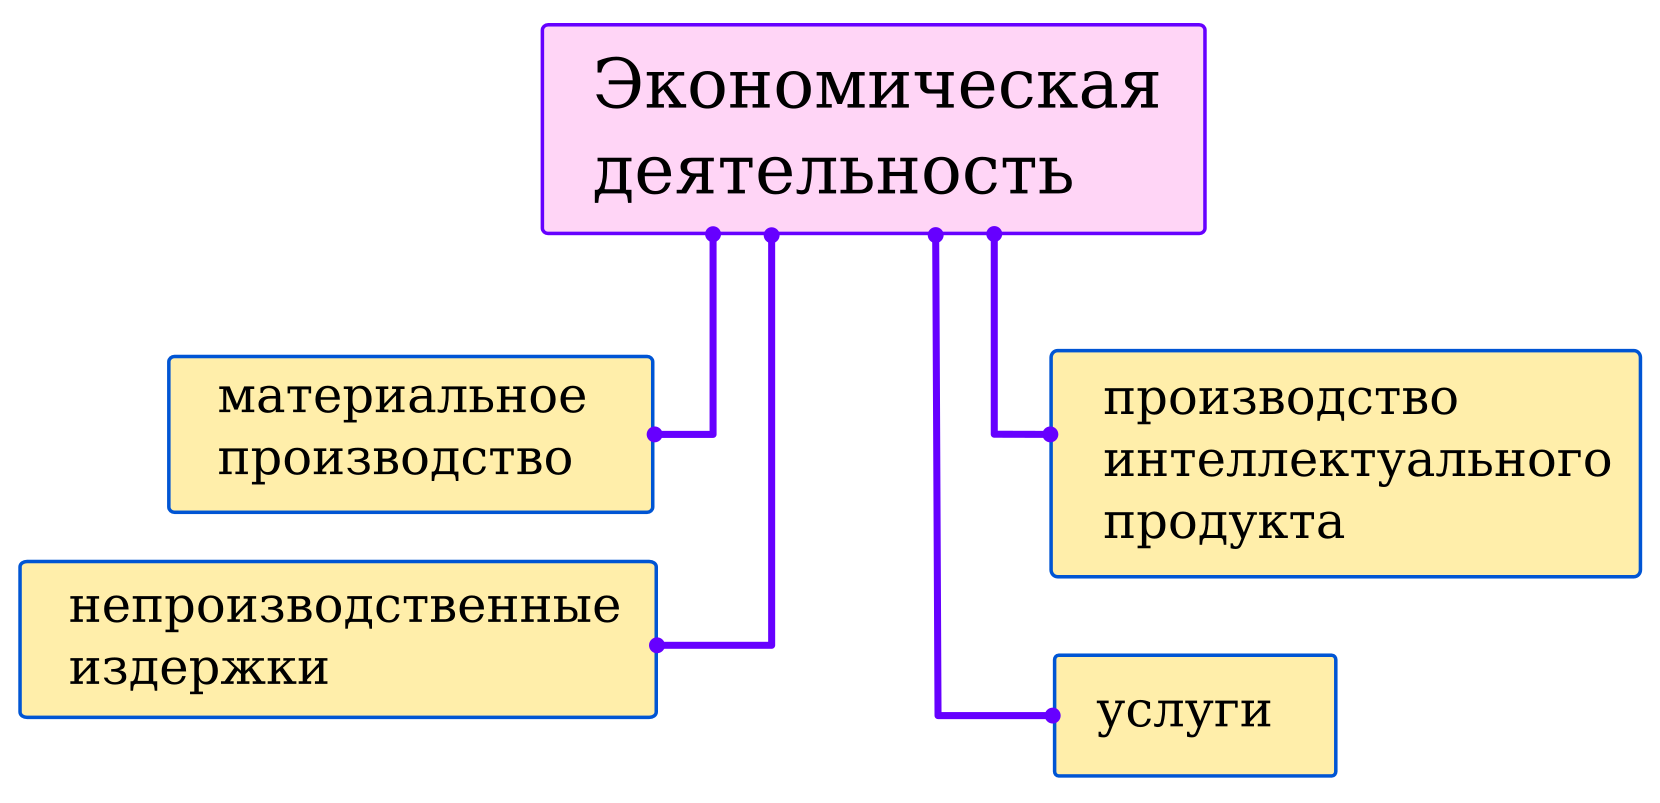
\includegraphics[width=0.70\textwidth]{eco-acts}
    \caption{Виды экономической деятельности}
    \label{fig:eco_acts}
\end{figure}

% команда \chapter недоступна в documentclass article
%\chapter{Повышение производительности труда на производстве}
\section*{Повышение производительности труда на производстве}

В случае с материальным производством программное обеспечение может быть внедрено и работать в составе аппаратно-программной платформы — производственной линии, промышленного робота, сельскохозяйственного робота, строительного робота, станка, транспортного средства, системы централизованного управления оборудованием или другого оборудования с элементами программного управления. Производственное предприятие интересует цена нового закупаемого оборудования как средства производства, которое позволяет создавать новую продукцию или повышает производительность труда на существующем производстве: экономический эффект от внедрения станка должен через некоторое время окупить его покупку.

Если программное обеспечение в составе аппаратно-программной платформы не лицензируется конечному потребителю за отдельную цену, стоимость его разработки будет компенсирована производителю оборудования из прибыли от проданного оборудования.

Возможна ситуация, когда для функционирования или эксплуатации оборудования необходимо лицензировать дополнительное программное обеспечение — к примеру, операционную систему на управляющем системном блоке, или специальное управляющее станком типовое программное обеспечение. Разработчиком и поставщиком программного обеспечения может выступать третья сторона или сам производитель оборудования, который решил не включать необходимое ПО в базовую поставку аппаратной платформы. В таком случае компенсация издержек на разработку такого программного обеспечения перекладывается на конечного потребителя оборудования через механизм покупки лицензий.

Стоимость производственного оборудования присоединяется к стоимости производимого продукта через механизм амортизации. Цена лицензии на дополнительное программное обеспечение компенсируется из прибыли. С точки зрения потребителя оборудования — производственного предприятия, необходимость покупки лицензии на программное обеспечение для того, чтобы оборудование можно было эксплуатировать, увеличивает цену этого оборудования на величину цены лицензий. Таким образом, оценивая целесообразность покупки оборудования, соизмеряя его цену и потенциальную выгоду от повышения производительности труда после его внедрения, он должен учитывать цену лицензий на необходимое программное обеспечение.

Внутренние прошивки микроконтроллеров обычно поставляются в качестве неотъемлемой части аппаратно-программной платформы (встроенное программное обеспечение, firmware). За отдельную лицензионную плату могут предлагать стороннее программное обеспечение — например, лицензию на операционную систему (лицензии ОС Microsoft Windows в варианте OEM или «коробочной» версии) или программные терминалы для управления оборудованием (системы CAM — computer-aided manufacturing)\footnote{Global CNC Software Market Status and Outlook 2022-2027 \cite{cncSoftMarketStatus2022}}. Более сложные комплексные решения, к примеру, системы мониторинга оборудования предприятия, могут одновременно включать как специально разработанные поставщиком программные и аппаратные модули, так и программные и аппаратные модули общего назначения сторонних производителей\footnote{Высоконагруженная распределенная система управления современной АЭС, Вадим Подольный \cite{highloadAes2018}}\footnote{SCADA Market Size, Analysis, Global Forecast by 2031 \cite{scadaMarket2023}}.

При единовременной закупке и внедрении программно-аппаратного комплекса сложно определить отдельно роль вклада улучшенной аппаратной части и роль вклада усовершенствованных программных алгоритмов в суммарное повышение производительности труда. Поэтому рассмотрим отдельно ситуацию, когда новое программное обеспечение внедряется на производство без привязки к закупке нового оборудования: не входит в состав аппаратно-программной платформы и не является необходимым условием минимальной эксплуатации станка. Возможные примеры: переключение между конкурирующими программными терминалами управления оборудованием\footnote{Global CNC Software Market Status and Outlook 2022-2027 \cite{cncSoftMarketStatus2022}}, установка новой версии используемого программного терминала с существенными улучшениями или установка дополнительных программных расширений к используемому терминалу; перевод процесса изготовления типовой детали с ручного оборудования в цифровой вид на имеющийся в распоряжении станок с ЧПУ или оптимизация существующего цифрового кода изготовления детали\footnote{Повышение производительности работы станков с числовым программным управлением и точности обработки деталей, Е. В. Сидорчик \cite{cncPerfomance2013}}; организация системы централизованного удаленного управления существующим парком станков поверх существующей сетевой инфраструктуры.

В этом случае внедрение нового программного обеспечения не привязано к закупке нового аппаратного обеспечения («железа») — оно разворачивается поверх существующего парка оборудования, речь идёт об установке «чистого» ПО. При этом его разработка и внедрение требует вложения известного количества ресурсов. Производственное предприятие может направить их на внутреннюю команду разработчиков или купить результат у 3-й стороны\footnote{IT-отдел, который приносит прибыль, а не убытки — вот как его организовать, Алексей Феофанов \cite{itProfit2023}}. Так или иначе, как при закупке нового оборудования, так и при направлении ресурсов на внедрение нового ПО, предприятие должно ответить на вопросы — каким будет масштаб расходов на внедрение и каким будет экономический эффект по результатам внедрения.

Результатом внедрения программного обеспечения на производстве должно стать повышение производительности производственного труда: уменьшение времени простоя оборудования, уменьшение процента брака, сокращение расхода энергии и сырых материалов (Рис. \ref{fig:effect_raw_materials}), необходимых для производства единицы продукции, сокращение количества необходимого труда рабочего в пересчете на единицу продукции\footnote{KUKA.EqualizingTech \cite{kukaEqulizingTech}}\footnote{Cummins ADEPT (Advanced Dynamic Efficient Powertrain Technology) \cite{cumminsAdept}}\footnote{Экономические, экологические и социальные эффекты цифровизации сельского хозяйства (на примере растениеводства), Н. Ю. Нестеренко, М. А. Ветрова \cite{agricultureEcoEffects2020}} и т. п. Так или иначе, это приведет к уменьшению индивидуальной стоимости продукции предприятия: больше продукта при старых затратах (Рис. \ref{fig:effect_manufacturing}(a)) или тот же продукт при меньших затратах (Рис. \ref{fig:effect_manufacturing}(б)). Выгода (экономический эффект) от внедрения ПО — добавочная прибыль, т. е. дополнительные средства, которые не появились бы в распоряжении собственников предприятия в том случае, если бы они не внедрили новое ПО, которое, действительно, привело к повышению производительности труда. Эта выгода может быть направлена на увеличение прибыли в денежном выражении (сверхприбыль), понижение цены готового продукта (захват рынка), повышение заработной платы рабочим, сокращение рабочего дня\footnote{Об исследованиях закономерного характера, факторов, эффектов и перспектив динамики рабочего времени в современной экономике, А. В. Золотов \cite{workingTime2020}} или распределена частями между всеми вариантами.

При рассмотрении варианта направления ресурсов на закупку или разработку и внедрение нового программного обеспечения, соизмеримость этих исходных затрат и предполагаемого экономического эффекта (добавочной прибыли) от внедрения — объективный критерий целесообразности реализации такого проекта. Добавочная прибыль — экономический эффект от внедрения программного обеспечения, — должна окупить издержки на покупку, разработку и внедрение этого программного обеспечения. После того, как исходные издержки были компенсированы, всю последующую добавочную прибыль можно рассматривать как чистый добавочный доход.

Стоимость реализации проекта по разработке ПО — величина фиксированная. Экономический эффект от внедрения будет тем больше, чем шире внедрена разработка. Эффект от цифровизации производства изделий, производимых в малом количестве, скорее всего не окупит первоначальных издержек на разработку. Цифровизация производства изделий, производимых большой серией, даст больший эффект. Максимальный эффект будет достигнут в масштабах общества — если программная разработка внедрена на множестве предприятий или внутри одного предприятия-монополиста, занимающего заметную долю мирового рынка (крупные производственные предприятия могут содержать собственные отделы по разработке ПО исключительно для внутреннего применения)\footnote{«Роснефть» разработала уникальные программы для цифрового изучения пород, Татьяна Романова \cite{rosneftSoftware2022}}\footnote{Программное обеспечение «Роснефти» гарантирует отрасли цифровой суверенитет, Татьяна Астафьева \cite{rosneftSoftware2023}}\footnote{Цифровая трансформация субъектов российской экономики в контексте достижения социально-экономического эффекта \cite{digitalTransformRus2021}}.

% картинки перемещаю в конец раздела, т.к. генератор pdf все равно раскидывает их по страницам и они не появляются между теми абзацами,
% где размещены изначально
\begin{figure}[h]
    \centering
    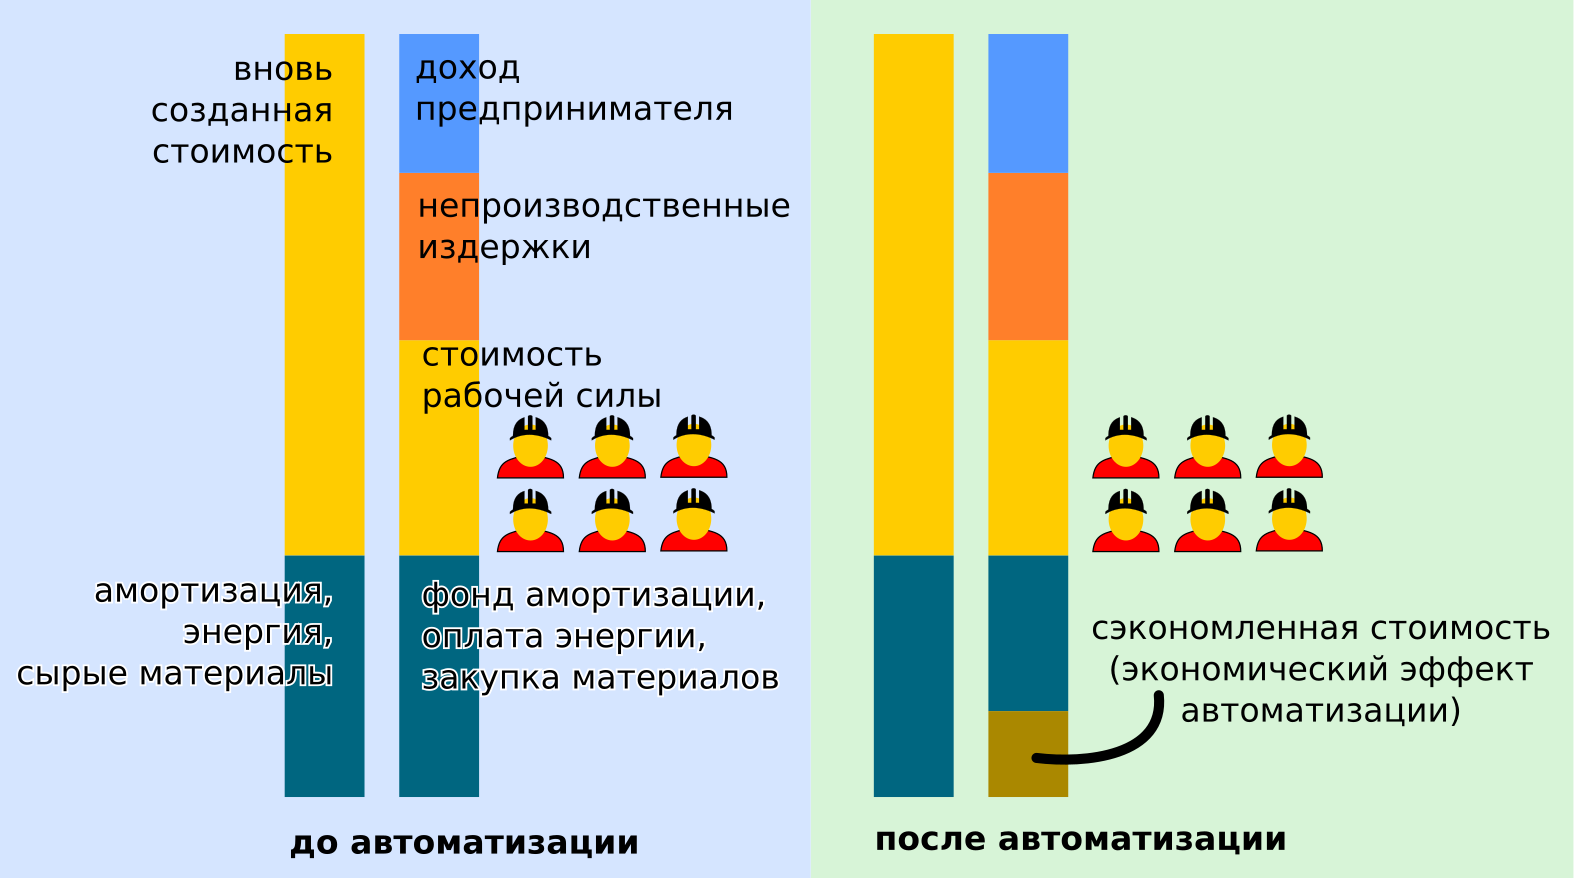
\includegraphics[width=0.70\textwidth]{effect-raw-materials}
    \caption{Экономический эффект автоматизации на производстве: сокращение расхода энергии, износа оборудования, расхода сырых материалов}
    \label{fig:effect_raw_materials}
\end{figure}

\begin{figure}[h]
    \centering
    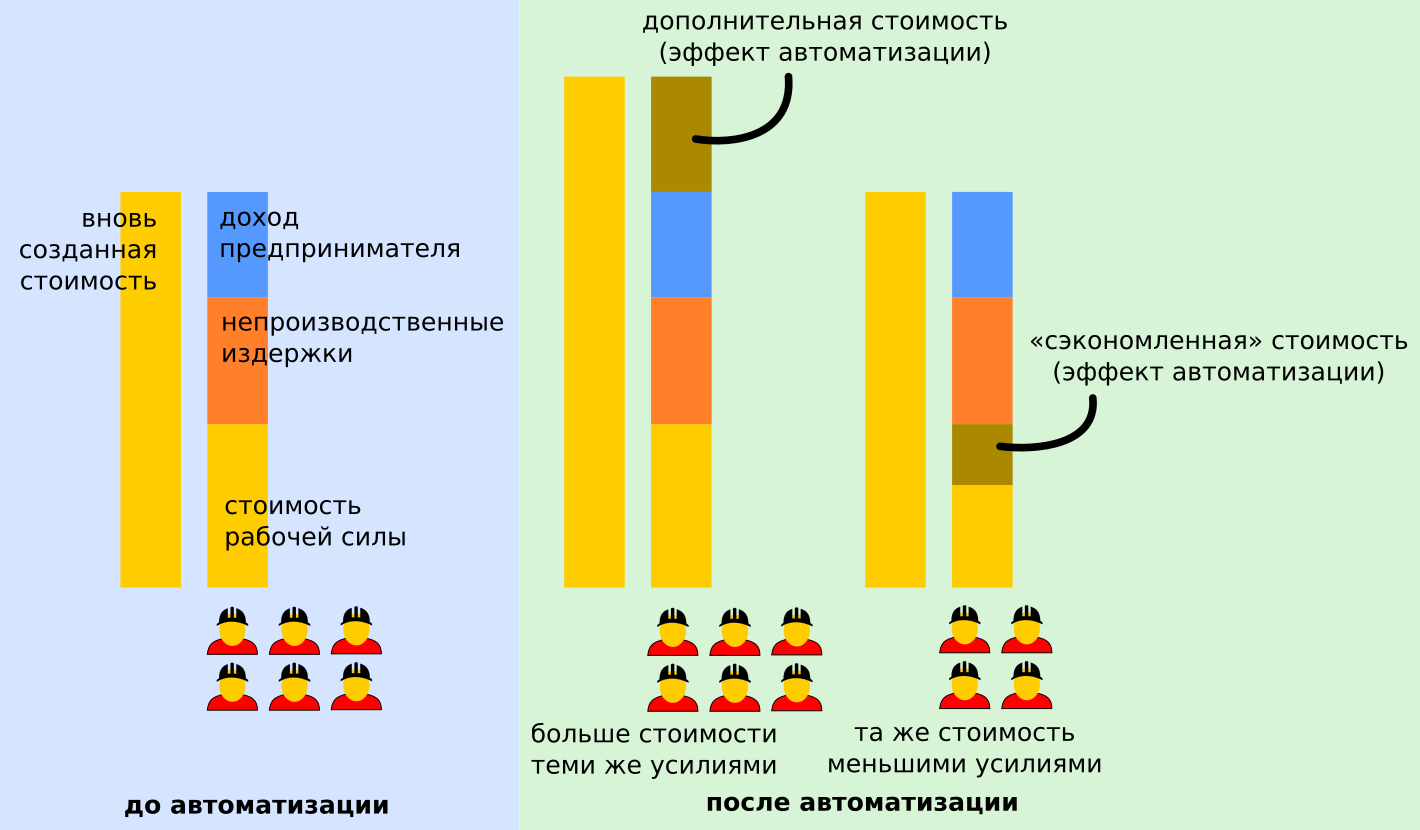
\includegraphics[width=0.70\textwidth]{effect-manufacturing}
    \caption{Экономический эффект автоматизации на производстве: (а) больше продукта старыми силами, (б) тот же продукт меньшими силами}
    \label{fig:effect_manufacturing}
\end{figure}

\section*{Сокращение непроизводственных издержек}

Непроизводственные издержки производственных предприятий или текущая деятельность предприятий, изначально не связанных с материальным производством.

Текущая деятельность сотрудников предприятия, не принимающих участия непосредственно в производстве, — руководство, бухгалтерия, юристы, HR, закупки, продажи и т. п. Аппаратно-программное обеспечение — ИТ-инфраструктура организации: персональные компьютеры, сеть, офисная техника. Базовый комплект программного обеспечения: офисное ПО, веб-браузер, электронная почта, мессенджер и т. п. Системы планирования ресурсов предприятия (ERP): оперативный учет, бухгалтерия, документооборот, CRM, управление проектами\footnote{Проектные способы выявления экономического эффекта от внедрения информационно-коммуникационных систем управления \cite{projectDetectEcoEffect2018}} и т. п. Настольные базы данных: справочно-правовые системы, государственные информационные системы, электронные каталоги, другие информационные системы. Решения на основе технологий работы с большими данными, алгоритмами машинного обучения и искусственного интеллекта (для крупных игроков, имеющих в распоряжении массивы данных соответствующих размеров\footnote{Греф заявил о миллиардных потерях Сбербанка из-за искусственного интеллекта \cite{sberAiLoss2019}}): повышение эффективности рекламных кампаний\footnote{Роль маркетинговых инноваций в повышении конкурентоспособности предприятия \cite{marketingInnovate2023}}), удержание пользователей, исследование поведения покупателей и т. п.

Без систем автоматизации издержки окажутся слишком велики. Очевидный вариант — сравнить процесс ведения бухгалтерии и сдачи отчетности на среднем предприятии на бумаге или в специализированном ПО: обычно даже простейшая автоматизация даёт преимущество по сравнению с ручным трудом. Но производительность может отличаться при работе с разными пакетами ПО или с разными поколениями одного и того же пакета цифрового ПО. Речь не обязательно может идти о повышении производительности труда в существующей организации: если новая организация не закупит типовой комплект офисного оборудования и лицензий на ПО, необходимый для ведения текущей деятельности, она не сможет держать издержки на среднем уровне по отрасли (Рис. \ref{fig:effect_nonproduction_normal}) и при прочих равных в конечном итоге проиграет конкурентам.

Внедрение новых систем автоматизации — еще большая  экономия по сравнению с уже имеющейся (Рис. \ref{fig:effect_nonproduction}): прежнее количество людей будет выполнять ту же работу за меньший срок или меньшее количество людей будут выполнять прежнюю работу за то же время.

Повышение производительности труда непроизводительных работников не повышает количество вновь созданного продукта, не увеличивает прибыль, но позволяет привлекать меньшее количество ресурсов для выполнения обычных задач, без которых предприятие не сможет нормально вести деятельность. Сокращая непроизводственные издержки, можно увеличивать долю прибыли, приходящуюся на предпринимательский доход, сокращая необходимые расходы. Или привести их к известному среднему уровню, чтобы их можно было покрывать прибылью от текущей деятельности в обычном режиме работы, сложившемся в отрасли. Эффект автоматизации может также быть выражен в высвобождении дополнительного рабочего времени имеющихся сотрудников так, что оно может быть использовано для реализации нового проекта\footnote{Греф рассказал о сокращениях в Сбербанке из-за искусственного интеллекта \cite{sberAiJobcut2018}}, который иначе бы не был реализован, или для снижения интенсивности рабочей нагрузки — увеличение свободного времени для самостоятельного развития и отдыха при прежних расходах и прежнем количестве выполненных задач.

В том случае, если речь идет о непроизводственной организации, к примеру, ведущей бухгалтерский учет или решающей юридические вопросы для других организаций на аутсорсе, повышение производительности такого профильного труда может увеличить выручку компании при неизменном количестве профильных сотрудников и тех же расходах на их зарплату, т. к. внедренные инструменты цифровой автоматизации позволят обслужить большее количество клиентов прежними силами. Таким образом, в масштабах организации речь идет не об экономии, а о наращивании «производства» реализованных непроизводственных проектов — прежнее количество человек будет решать большее количество задач. Однако в масштабах экономики всё равно произойдет экономия труда, направленного на решение задачи автоматизированной этим способом, т. к. предприятия выносят решение задач на аутсорсинг с такой целью, чтобы тратить меньшее количество ресурсов на решение этих же задач у себя.

Системы мониторинга и сбора статистики с производственного оборудования\footnote{Системы мониторинга станков с ЧПУ в России Обзор технологий и рынка \cite{cncMonitoringRus2016}}\footnote{Global CNC Machine Monitoring Software Market Research Report 2022 \cite{cncMonitoringGlobal2022}} и системы автоматического учета рабочего времени не повышает напрямую производительность производственного труда рабочих, но автоматизируют и повышают эффективность труда по управлению производственным процессом — руководство, менеджеры, производственные аналитики. Целью такого труда является поддержание производительности производственного процесса на целевом уровне, к примеру, через контроль за соблюдением установленных регламентов, а также выявление на производстве узких мест и разработка новых регламентов, которые, к примеру, позволят сократить простои оборудования, таким образом в итоге повысив общую целевую производственную производительность. Цифровые системы учета рабочего времени снимают нагрузку с линейных руководителей, осуществляющих контроль производственного процесса. Цифровые системы мониторинга оборудования позволяют получить достоверную картину производственного процесса, обновляемую в реальном времени. Собранные данные составляют информационный фундамент для принятия решений (руководство), проработки и реализации проектов по реорганизации производственного процесса так, чтобы производительность производственного труда в итоге повысилась (производственные аналитики)\footnote{Assessment of Economic Efficiency, Effects and Risks of Digitalization Projects of Garment Industry in Russia \cite{garminIndustryEcoEffect2023}}\footnote{Управление процессом установления норм труда с применением статистических информационных систем \cite{laborStandards2017}}. Таким образом финальная цель внедрения такой системы — получение добавочной прибыли — экономического эффекта от сокращения издержек и повышения производительности, но, в отличие от систем непосредственной автоматизации производства, в том числе систем централизованного управления оборудованием, включающих функции мониторинга, она реализуется опосредованно через реализацию проектов производственных аналитиков и решения руководства.

Основа системы мониторинга производственного оборудования обычно — увесистая распределенная программная платформа, включающая модули сбора информации, базу данных, интерфейс мониторинга, генераторы отчетов и прочие. Но она также может включать аппаратную составляющую — специальные устройства (например, датчики для сбора информации со станка) и устройства общего назначения (как минимум, сетевая инфраструктура и серверы достаточной производительности).

% картинки перемещаю в конец раздела, т.к. генератор pdf все равно раскидывает их по страницам и они не появляются между теми абзацами,
% где размещены изначально
\begin{figure}[h]
    \centering
    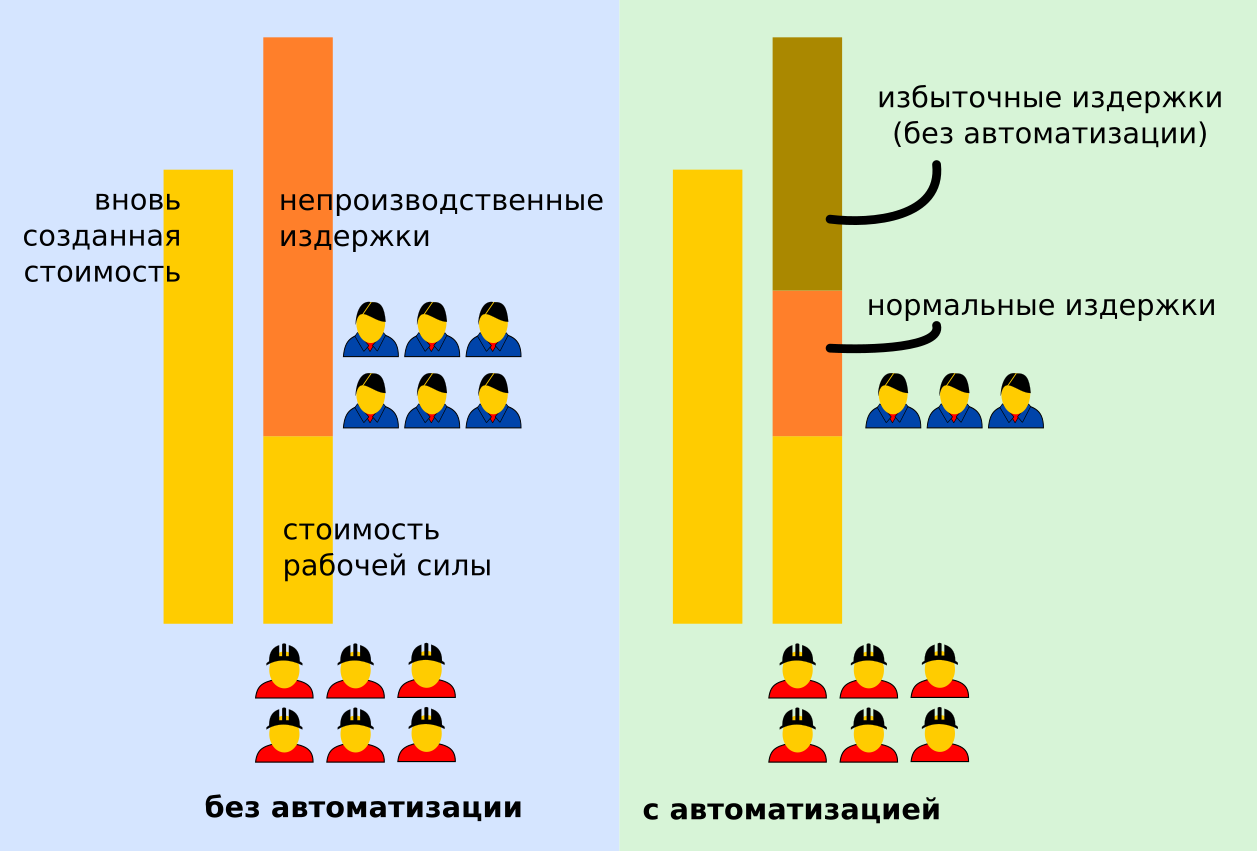
\includegraphics[width=0.70\textwidth]{effect-nonproduction-normal}
    \caption{Экономический эффект автоматизации непроизводственных издержек: избыточные издержки по сравнению с нормальным уровнем в среднем по отрасли}
    \label{fig:effect_nonproduction_normal}
\end{figure}

\begin{figure}[h]
    \centering
    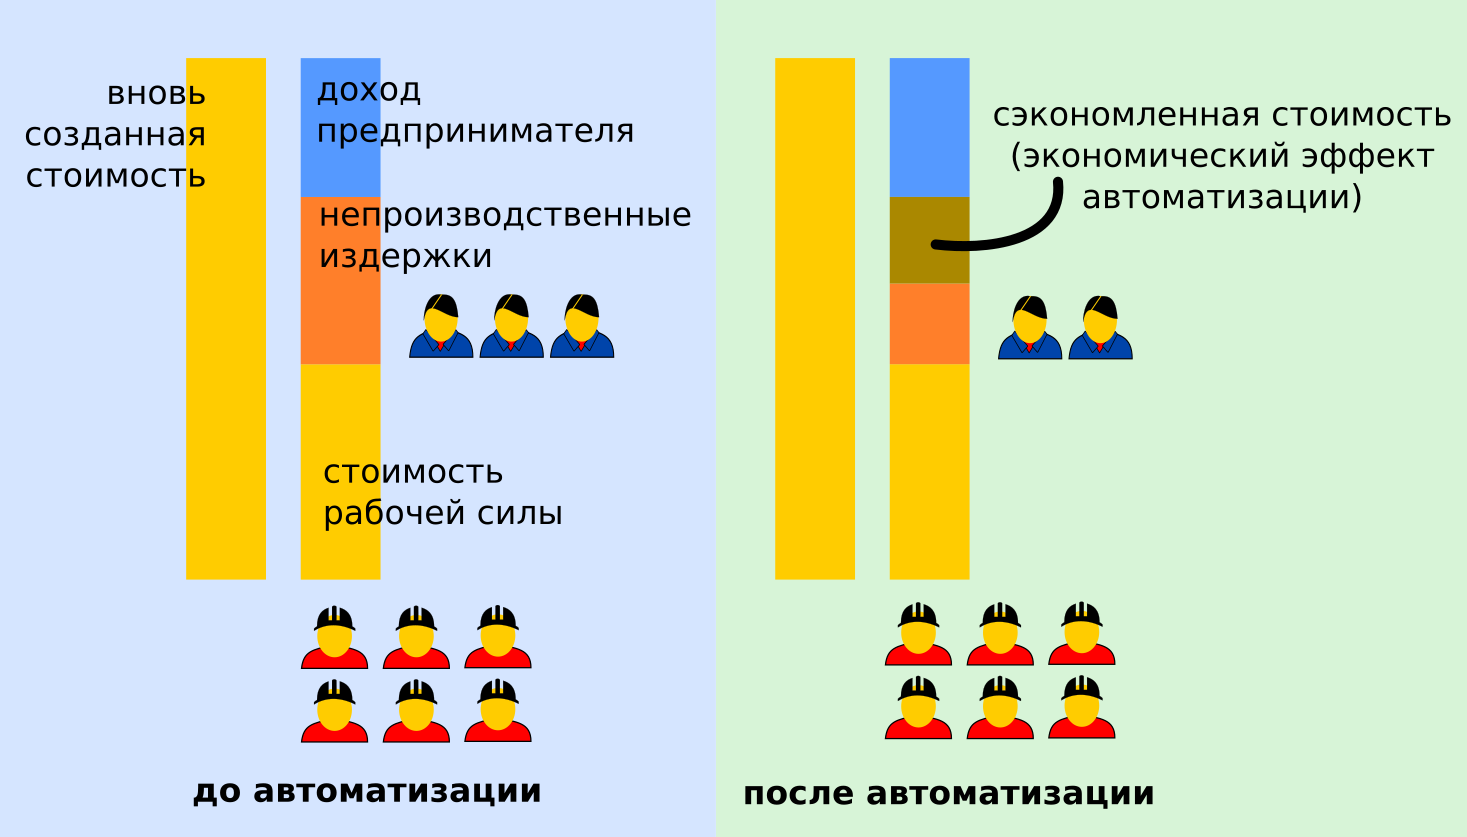
\includegraphics[width=0.70\textwidth]{effect-nonproduction}
    \caption{Экономический эффект автоматизации непроизводственных издержек: сокращение необходимых издержек}
    \label{fig:effect_nonproduction}
\end{figure}

\section*{Государственные услуги — непроизводственные издержки в масштабах общества}

В качестве особого случая сокращения непроизводственных издержек рассмотрим проекты цифровой автоматизации государственных услуг: портал Госуслуги, приём электронных заявок от граждан на сайтах специальных государственных учреждений и министерств (ФНС, ГИБДД), сайтах муниципалитетов и т. п. Программное обеспечение такого рода повышает производительность труда чиновников — это непроизводственные издержки в масштабах общества. Это экономия ресурсов, большее количество решенных задач\footnote{Model of creating an economic ecosystem in the framework of economic convergence under the influence of digitalization \cite{economicEcosystem2021}}. Повышение производительности труда чиновников также приводит к тому, что процедуры решения вопросов, требующих взаимодействия с населением, будут требовать меньше времени участия и самих граждан: сокращение времени на заполнение электронной заявки, уменьшение количества ситуаций, требующих личного присутствия в организации, отсутствие необходимости ожидания в живых очередях. Таким образом, у граждан высвободится свободное время, которое они смогут потратить на отдых, развитие, общение в семье, социализацию, хобби — это улучшение качества жизни, пополнение общественного фонда свободного времени. В этом случае можно говорить не только об экономическом, но и о социальном эффекте от внедрения такого рода систем цифровой автоматизации.

Экономический и социальный эффект от внедрения очередного цифрового государственного сервиса будет тем выше, чем больше государственных чиновников и граждан в него вовлечены, чем чаще граждане вынуждены к нему обращаться, чем больше текущая процедура решения вопроса занимает времени.

Внедрение цифровых государственных сервисов, как и любое сокращение издержек, не может увеличить абсолютное богатство государства или региона самим фактом своего внедрения. Однако оно может высвободить ресурсы, которые в конечном итоге создадут в государстве или регионе дополнительные блага. Сокращение издержек может быть выражено в денежном эквиваленте — экономия бюджета при решении тех же самых необходимых задач; в высвобождении рабочего времени аппарата чиновников, которое может быть потрачено на решение дополнительной массы задач, которые в противном случае не были бы решены; в высвобождении свободного времени граждан, т. е., в конечном итоге, в повышении качества жизни.

\section*{Автоматизация услуг}

Под оказанием услуги здесь будем понимать такой труд, предметом которого является непосредственно человек: развлечения, индустрия красоты, спорт, образование, медицина, пассажирские перевозки.

Средствами цифровой автоматизации могут служить аппаратно-программные платформы, облачные технологии, «чистое» ПО, устанавливаемое на типовой персональный компьютер, смартфон или планшет.

Прямые трансляции через интернет и социальные сети позволяют повысить охват, т. е. распространить, к примеру, образовательную или развлекательную услугу фактически на неограниченное количество потребителей. Однако сценарии оказания услуги, при которых требуется индивидуальный подход и обратная связь, накладывают существенные ограничения на повышение производительности труда, т. е. на количество потребителей, которые могут получить услугу в заданный отрезок времени.

Средства автоматизации медицинских услуг — медицинское оборудование, электронные медицинские карты пациентов, облачные системы мониторинга физиологических показателей пациентов, рекомендательные системы на основе алгоритмов искусственного интеллекта\footnote{IBM Watson Health \cite{ibmWatson2022}}. Современное медицинское диагностическое оборудование обычно представляет собой аппаратно-программную платформу с встроенным и внешним управляющим программным обеспечением, а также со специальным программным обеспечением, необходимым для того, чтобы просмотреть и проанализировать полученный с прибора результат. Инструменты позволяют повысить качество обслуживания — получить медицинские показатели пациента, на основе которых можно поставить более точный диагноз, в некоторых случаях — сократить время, необходимое для индивидуальной работы с пациентом, т. е. в прямом простом смысле повысить производительность труда. В масштабах экономики действительное качество медицинского обслуживания, в т. ч. раннее выявление болезней и профилактика, обеспечивает трудоспособность занятой в системе производства рабочей силы.

При оказании образовательной услуги обратную связь предполагают: проверка индивидуальных заданий, проведение промежуточных опросов, проведение практических занятий, проведение занятий, предполагающих совместное обсуждение, ответы на уточняющие вопросы во время общей лекции, руководство индивидуальными проектами, финальная проверка знаний — приём зачета, экзамена, индивидуального квалификационного проекта. Средства автоматизации не могут радикально уменьшить необходимое время индивидуального взаимодействия преподавателя и обучающегося, но позволяют сократить часть рутины. Электронный дневник — сокращение работы, необходимой для ведения журнала посещений и текущей успеваемости, электронные программы автоматического тестирования — проверка минимального набора знаний и умений, система «антиплагиат» — сокращение времени на проверку индивидуальных творческих проектов. Инструменты дистанционного обучения при работе из дома сокращают время на дорогу до рабочего помещения, сокращают издержки на содержание рабочего помещения — уборка, электричество (в действительности, перекладывают их на преподавателя, личное жильё которого начинает отчасти выполнять роль учебной аудитории). Если работа преподавателя ведется из специально подготовленной аудитории, то это просто экономия средств на содержании помещения: аудитория не должна вмещать учебную группу, т. е. может быть рассчитана на значительно меньшее количество человек; дополнительные расходы — техническое оборудование для ведения трансляции, надежный широкий канал доступа в интернет, дополнительная  нагрузка на системного администратора.

Платформы массового онлайн-образования такие, как Курсера\footnote{How Coursera Makes Money \cite{howCourseraMakesMoney2022}}, позволяют провайдерам услуги загружать записи лекций, превращая таким образом эту часть услуги в форму распространения контента. Вместе с тем оставляют возможность для преподавателя принимать участие в образовательном процессе отдельных учеников — отвечать на вопросы, проверять домашние задания, принимать экзамен (обычно в форме выпускного проекта). Инструменты автоматизации обратной связи: отображение индивидуального прогресса обучения — встроено в сайт; квизы между лекциями, квизы, встроенные в запись лекции, — анкеты с заранее известными ответами, полностью автоматизированы; чат с преподавателем, проверка индивидуальной работы преподавателем, взаимная проверка индивидуальных работ участниками курса (peer-review) — обратная связь с участием живого человека посредством цифровых инструментов. Взаимная проверка работ (peer-review) — перекладывание индивидуальной обратной связи с преподавателя на самих студентов под видом элемента образовательного процесса. Провайдер услуги несет единовременные первоначальные издержки на создание образовательного контента — запись лекций, составление списка вопросов и ответов для квизов, приведение их в специальный формат, загрузка на портал. После запуска курса общая сумма подписки компенсирует на постоянной основе: стоимость облачной инфраструктуры (аппаратное обеспечение, электричество, труд системных администраторов) и стоимость, собственно, услуги — труд преподавателей в объеме, предусмотренном механизмами обратной связи. В каком объеме будет предоставлена обратная связь, решает провайдер услуги — партнер платформы. Платформы массового онлайн-образования позволяют привлекать к опубликованным курсам достаточно широкую аудиторию со всего мира, гораздо более широкую, чем обычная учебная группа, посещающая в традиционном режиме оффлайн университет. Просмотр записанных лекций и решение автоматических квизов масштабируется на любое количество студентов — ограничения накладывают только аппаратные возможности облачной инфраструктуры. Необходимость живой обратной связи от преподавателя накладывает существенное ограничение на масштаб аудитории, которая может пройти через курс в режиме онлайн. По этой причине провайдеры услуги стараются минимизировать её количество в процессе курса или полностью от нее отказываются, оставляя только автоматические тесты и взаимные проверки peer-review. В том случае, если живая обратная связь со стороны преподавателя не предусмотрена совсем, образовательная услуга вырождается в механизм предоставления средств для самообразования — самостоятельного индивидуального потребления специального образовательного контента; платформа онлайн-образования из платформы оказания образовательных услуг превращается в платформу распространения и потребления цифрового образовательного контента (своеобразную электронную библиотеку). Наличие курсов, не предполагающих обратную связь преподавателей (в т. ч. курсы с включенным механизмом peer-review), позволяет увеличить охват платформы, в т. ч. предоставляя бесплатный доступ к части такого контента\footnote{COURSERA, INC., Form S-1 REGISTRATION STATEMENT Under The Securities Act of 1933 \cite{courseraS1}}.

\section*{Инженерное программное обеспечение — повышение производительности труда, создающего интеллектуальный продукт}

Программное обеспечение для инженерных разработок, в т.ч. программное обеспечение для разработки программного обеспечения. Системы автоматического проектирования (САПР), пакеты математических вычислений, пакеты компьютерной симуляции, редакторы компьютерной графики (векторной, растровой, 2д, 3д), системы прототипирования, макетирования и проектирования программного обеспечения, САПР для проектирования микроэлектроники (EDA — electronic design automation), специализированные редакторы диаграмм, компиляторы языков программирования низкого и высокого уровня, системы для отладки приложений, простые редакторы кода, интегрированные среды разработки, программные библиотеки, библиотеки цифровых аппаратных модулей на языках описания аппаратного обеспечения, субд, инфраструктурные платформы и фреймворки, системы управления исходным кодом, системы разработки в команде, системы управления проектами, системы no-code, системы генерации изображений, кода, прочего контента на основе нейросетевых алгоритмов.
Повышают производительность труда инженеров, дизайнеров, исследователей, ученых в области любых инженерных и исследовательских разработок, в том числе в области разработки программного обеспечения. Экономия ресурсов на этапах разработки, эксплуатации, поддержки проектов: сокращение времени на разработку типовых инженерных проектов до их внедрения, сокращение минимальной команды, необходимой для разработки типовых инженерных проектов, сокращение времени изучения новых инструментов специалистами, понижение планки входа в индустрию для специалистов, усложнение типовых инженерных проектов.
Развитие индустрии технологий цифровой разработки в целом ведет к сокращению издержек на реализацию научно-технических проектов (экономический эффект первого порядка), что в конечном итоге приводит к удешевлению, расширению и ускорению процессов цифровой автоматизации во всех остальных областях экономики (действительный экономический эффект), в том числе в самой области разработки инструментов для инженерных разработок. В том случае, если сэкономленные в результате повышения производительности инженерного труда средства будут повторно направлены на дополнительные инженерные разработки, можно говорить о добавочном повышении производительности труда и производном от него добавочном действительном экономическом эффекте. Максимальный экономический эффект первого порядка будет достигнут в местах сосредоточения инженерных, исследовательских и прочих команд, занятых в области реализации инженерных технологических проектов — в экономиках, выделяющих значительный объем ресурсов на развитие существующих и запуск новых технологических проектов. Действительный экономический эффект будет реализован в экономиках, внедряющих научно-технические разработки на действующих предприятиях.

%1. Population and Area (Historical Censuses) // United States Census Bureau. [Электронный ресурс]. – URL: http://www2.census.gov/prod2/statcomp/documents/1991-02.pdf
%2. The Punched Card Tabulator, IBM’s 100 Icons of Progress [Электронный ресурс]. – URL: https://www.ibm.com/ibm/history/ibm100/us/en/icons/tabulator/
%3. The Hollerith tabulating machine in business office / S. G. Koon. // Machinery, Сентябрь 1913, - С. 25 - [Электронный ресурс]. – URL: http://archive.org/details/sim_machinery_1913-09/page/24/
%4. Organizing for work / H. L. Gantt // Harcourt, Brace and Howe, New York, - 1919. [Электронный ресурс]. – URL: https://archive.org/details/organizingforwor00gant
%5. Global CNC Software Market Status and Outlook 2022-2027 // 360 Market Updates, – 2022. [Электронный ресурс]. – URL: https://www.360marketupdates.com/global-cnc-software-market-21107093
%6. Высоконагруженная распределенная система управления современной АЭС / Вадим Подольный // HighLoad++, Москва, СКОЛКОВО, – 2018. [Электронный ресурс]. – URL: https://highload.ru/moscow/2018/abstracts/4339
%7. SCADA Market Size, Analysis, Global Forecast by 2031 // MarketsandMarkets, – 2023. [Электронный ресурс]. – URL: https://www.marketsandmarkets.com/Market-Reports/scada-market-19487518.html
%8. Сидорчик, Е. В. Повышение производительности работы станков с числовым программным управлением и точности обработки деталей / Е. В. Сидорчик // Интернет-журнал Науковедение. – 2013. – № 4(17). – С. 67. – EDN RSHECB.
%9. IT-отдел, который приносит прибыль, а не убытки — вот как его организовать. / Алексей Феофанов. // RB.RU, – 2023. [Электронный ресурс]. – URL: https://rb.ru/opinion/it-workcheck/
%10. KUKA.EqualizingTech // KUKA. [Электронный ресурс]. – URL: https://www.kuka.com/en-us/products/robotics-systems/software/application-software/kuka_equalizingtech
%11. Cummins ADEPT (Advanced Dynamic Efficient Powertrain Technology) // Cummins. [Электронный ресурс]. – URL: https://www.cummins.com/support/digital-products-and-services-support/adept-support
%12. Нестеренко, Н. Ю. Экономические, экологические и социальные эффекты цифровизации сельского хозяйства (на примере растениеводства) / Н. Ю. Нестеренко, М. А. Ветрова // Международный экономический симпозиум - 2020 : Материалы международных научных конференций: «Устойчивое развитие: общество и экономика», «Соколовские чтения. Бухгалтерский учет: взгляд из прошлого в будущее», Санкт-Петербург, 01–30 июня 2020 года. – Санкт-Петербург: Санкт-Петербургский государственный университет, 2020. – С. 94-99. – EDN NOZCWA.
%13. Золотов, А. В. Об исследованиях закономерного характера, факторов, эффектов и перспектив динамики рабочего времени в современной экономике / А. В. Золотов // Народонаселение. – 2020. – Т. 23, № 3. – С. 155-168. – DOI 10.19181/population.2020.23.3.14. – EDN JYBSWO.
%14. «Роснефть» разработала уникальные программы для цифрового изучения пород / Татьяна Романова // Лента.Ру, – 2022. [Электронный ресурс]. – URL: https://lenta.ru/news/2022/08/01/model1/
%15. Программное обеспечение «Роснефти» гарантирует отрасли цифровой суверенитет / Татьяна Астафьева // Независимая газета, – 2023. [Электронный ресурс]. – URL: https://www.ng.ru/economics/2023-06-01/8_8739_01062023.html
%16. Цифровая трансформация субъектов российской экономики в контексте достижения социально-экономического эффекта / Э. Р. Горчакова, С. М. Макейкина, Е. А. Мамышева, П. О. Цыганов // Вестник Алтайской академии экономики и права. – 2021. – № 9-1. – С. 43-51. – DOI 10.17513/vaael.1837. – EDN NPRFEJ.
%17. Шангин, А. В. Проектные способы выявления экономического эффекта от внедрения информационно-коммуникационных систем управления / А. В. Шангин // Вестник Национального Института Бизнеса. – 2018. – № 33. – С. 104-110. – EDN IRAFXO.
%18. Греф заявил о миллиардных потерях Сбербанка из-за искусственного интеллекта // РИА Новости, – 2019. [Электронный ресурс]. – URL: https://ria.ru/20190226/1551377003.html
%19. Камчатова, Е. Ю. Роль маркетинговых инноваций в повышении конкурентоспособности предприятия / Е. Ю. Камчатова, В. В. Бурлаков, М. А. Яхъяев // Инновации и инвестиции. – 2023. – № 3. – С. 4-7. – EDN LGMUAR.
%20. Греф рассказал о сокращениях в Сбербанке из-за искусственного интеллекта / Георгий Тадтаев // РБК, – 2018. [Электронный ресурс]. – URL:  https://www.rbc.ru/business/10/11/2018/5be6b5929a79471263626f32
%21. Системы мониторинга станков с ЧПУ в России Обзор технологий и рынка / Ю. Куркова, А. Васильев, А. Ловыгин, В. Степанов // САПР и графика. – 2016. – № 12(242). – С. 24-31. – EDN ZFDETX.
%22. Global CNC Machine Monitoring Software Market Research Report 2022 - Market Size, Current Insights and Development Trends, Publishing Date : 02-Jun-2022 | No. of pages : 125, https://www.researchreportsworld.com/global-cnc-machine-monitoring-software-market-21003349
%23. Assessment of Economic Efficiency, Effects and Risks of Digitalization Projects of Garment Industry in Russia / T. Yu. Kudryavtseva, K. S. Kozhina, G. K. Prause, E. O. Olaniyi // Journal of Applied Economic Research. – 2023. – Vol. 22, No. 1. – P. 72-98. – DOI 10.15826/vestnik.2023.22.1.004. – EDN UISWXV.
%24. Кутимская, М. А. Управление процессом установления норм труда с применением статистических информационных систем / М. А. Кутимская, С. А. Сморчкова // Вестник Омского университета. Серия: Экономика. – 2017. – № 3(59). – С. 126-133. – DOI 10.25513/1812-3988.2017.3.126-133. – EDN ZUEXNT.
%25. Kalayda, S. A. Model of creating an economic ecosystem in the framework of economic convergence under the influence of digitalization / S. A. Kalayda // Journal of Applied Informatics. – 2021. – Vol. 16, No. 6(96). – P. 28-42. – DOI 10.37791/2687-0649-2021-16-6-28-42. – EDN CCFGNE.
%26. IBM Watson Health // TAdviser Zdrav.Expert. [Электронный ресурс]. – URL:  https://zdrav.expert/index.php/Продукт:IBM_Watson_Health
%27. How Coursera Makes Money / Jakob Eckstein // Investopedia, – 2022. [Электронный ресурс]. – URL: https://www.investopedia.com/articles/investing/042815/how-coursera-works-makes-money.asp
%28. COURSERA, INC., Form S-1 REGISTRATION STATEMENT Under The Securities Act of 1933 // U.S. Securities and Exchange Commission, – 2021. [Электронный ресурс]. – URL: https://www.sec.gov/Archives/edgar/data/1651562/000119312521071525/d65490ds1.htm


% чтобы ссылки в тексте имели правильные номера, генератор нужно запустить два раза
% нижние подчеркивания '_' в ссылках заменяем на '\_', иначе они воспринимаются как спец-символы
\begin{thebibliography}{2}
\bibitem{usCentus} Population and Area (Historical Censuses) // United States Census Bureau. [Электронный ресурс]. – URL: http://www2.census.gov/prod2/statcomp/documents/1991-02.pdf
\bibitem{ibmPuchCard} The Punched Card Tabulator, IBM’s 100 Icons of Progress [Электронный ресурс]. – URL: https://www.ibm.com/ibm/history/ibm100/us/en/icons/tabulator/
\bibitem{machinery1913} The Hollerith tabulating machine in business office / S. G. Koon. // Machinery, Сентябрь 1913, - С. 25 - [Электронный ресурс]. – URL: http://archive.org/details/sim\_machinery\_1913-09/page/24/
\bibitem{ecoEffectOrganizingForWork} Organizing for work / H. L. Gantt // Harcourt, Brace and Howe, New York, - 1919. [Электронный ресурс]. – URL: https://archive.org/details/organizingforwor00gant
\bibitem{cncSoftMarketStatus2022} Global CNC Software Market Status and Outlook 2022-2027 // 360 Market Updates, – 2022. [Электронный ресурс]. – URL: https://www.360marketupdates.com/global-cnc-software-market-21107093
\bibitem{highloadAes2018} Высоконагруженная распределенная система управления современной АЭС / Вадим Подольный // HighLoad++, Москва, СКОЛКОВО, – 2018. [Электронный ресурс]. – URL: https://highload.ru/moscow/2018/abstracts/4339
\bibitem{scadaMarket2023} SCADA Market Size, Analysis, Global Forecast by 2031 // MarketsandMarkets, – 2023. [Электронный ресурс]. – URL: https://www.marketsandmarkets.com/Market-Reports/scada-market-19487518.html
\bibitem{cncPerfomance2013} Сидорчик, Е. В. Повышение производительности работы станков с числовым программным управлением и точности обработки деталей / Е. В. Сидорчик // Интернет-журнал Науковедение. – 2013. – № 4(17). – С. 67. – EDN RSHECB.
\bibitem{itProfit2023} IT-отдел, который приносит прибыль, а не убытки — вот как его организовать. / Алексей Феофанов. // RB.RU, – 2023. [Электронный ресурс]. – URL: https://rb.ru/opinion/it-workcheck/
\bibitem{kukaEqulizingTech} KUKA.EqualizingTech // KUKA. [Электронный ресурс]. – URL: https://www.kuka.com/en-us/products/robotics-systems/software/application-software/kuka\_equalizingtech
\bibitem{cumminsAdept} Cummins ADEPT (Advanced Dynamic Efficient Powertrain Technology) // Cummins. [Электронный ресурс]. – URL: https://www.cummins.com/support/digital-products-and-services-support/adept-support
\bibitem{agricultureEcoEffects2020} Нестеренко, Н. Ю. Экономические, экологические и социальные эффекты цифровизации сельского хозяйства (на примере растениеводства) / Н. Ю. Нестеренко, М. А. Ветрова // Международный экономический симпозиум - 2020 : Материалы международных научных конференций: «Устойчивое развитие: общество и экономика», «Соколовские чтения. Бухгалтерский учет: взгляд из прошлого в будущее», Санкт-Петербург, 01–30 июня 2020 года. – Санкт-Петербург: Санкт-Петербургский государственный университет, 2020. – С. 94-99. – EDN NOZCWA.
\bibitem{workingTime2020} Золотов, А. В. Об исследованиях закономерного характера, факторов, эффектов и перспектив динамики рабочего времени в современной экономике / А. В. Золотов // Народонаселение. – 2020. – Т. 23, № 3. – С. 155-168. – DOI 10.19181/population.2020.23.3.14. – EDN JYBSWO.
\bibitem{rosneftSoftware2022} «Роснефть» разработала уникальные программы для цифрового изучения пород / Татьяна Романова // Лента.Ру, – 2022. [Электронный ресурс]. – URL: https://lenta.ru/news/2022/08/01/model1/
\bibitem{rosneftSoftware2023} Программное обеспечение «Роснефти» гарантирует отрасли цифровой суверенитет / Татьяна Астафьева // Независимая газета, – 2023. [Электронный ресурс]. – URL: https://www.ng.ru/economics/2023-06-01/8\_8739\_01062023.html
\bibitem{digitalTransformRus2021} Цифровая трансформация субъектов российской экономики в контексте достижения социально-экономического эффекта / Э. Р. Горчакова, С. М. Макейкина, Е. А. Мамышева, П. О. Цыганов // Вестник Алтайской академии экономики и права. – 2021. – № 9-1. – С. 43-51. – DOI 10.17513/vaael.1837. – EDN NPRFEJ.
\bibitem{projectDetectEcoEffect2018} Шангин, А. В. Проектные способы выявления экономического эффекта от внедрения информационно-коммуникационных систем управления / А. В. Шангин // Вестник Национального Института Бизнеса. – 2018. – № 33. – С. 104-110. – EDN IRAFXO.
\bibitem{sberAiLoss2019} Греф заявил о миллиардных потерях Сбербанка из-за искусственного интеллекта // РИА Новости, – 2019. [Электронный ресурс]. – URL: https://ria.ru/20190226/1551377003.html
\bibitem{marketingInnovate2023} Камчатова, Е. Ю. Роль маркетинговых инноваций в повышении конкурентоспособности предприятия / Е. Ю. Камчатова, В. В. Бурлаков, М. А. Яхъяев // Инновации и инвестиции. – 2023. – № 3. – С. 4-7. – EDN LGMUAR.
\bibitem{sberAiJobcut2018} Греф рассказал о сокращениях в Сбербанке из-за искусственного интеллекта / Георгий Тадтаев // РБК, – 2018. [Электронный ресурс]. – URL:  https://www.rbc.ru/business/10/11/2018/5be6b5929a79471263626f32
\bibitem{cncMonitoringRus2016} Системы мониторинга станков с ЧПУ в России Обзор технологий и рынка / Ю. Куркова, А. Васильев, А. Ловыгин, В. Степанов // САПР и графика. – 2016. – № 12(242). – С. 24-31. – EDN ZFDETX.
\bibitem{cncMonitoringGlobal2022} Global CNC Machine Monitoring Software Market Research Report 2022 - Market Size, Current Insights and Development Trends, Publishing Date : 02-Jun-2022 | No. of pages : 125, https://www.researchreportsworld.com/global-cnc-machine-monitoring-software-market-21003349
\bibitem{garminIndustryEcoEffect2023} Assessment of Economic Efficiency, Effects and Risks of Digitalization Projects of Garment Industry in Russia / T. Yu. Kudryavtseva, K. S. Kozhina, G. K. Prause, E. O. Olaniyi // Journal of Applied Economic Research. – 2023. – Vol. 22, No. 1. – P. 72-98. – DOI 10.15826/vestnik.2023.22.1.004. – EDN UISWXV.
\bibitem{laborStandards2017} Кутимская, М. А. Управление процессом установления норм труда с применением статистических информационных систем / М. А. Кутимская, С. А. Сморчкова // Вестник Омского университета. Серия: Экономика. – 2017. – № 3(59). – С. 126-133. – DOI 10.25513/1812-3988.2017.3.126-133. – EDN ZUEXNT.
\bibitem{economicEcosystem2021} Kalayda, S. A. Model of creating an economic ecosystem in the framework of economic convergence under the influence of digitalization / S. A. Kalayda // Journal of Applied Informatics. – 2021. – Vol. 16, No. 6(96). – P. 28-42. – DOI 10.37791/2687-0649-2021-16-6-28-42. – EDN CCFGNE.
\bibitem{ibmWatson2022} IBM Watson Health // TAdviser Zdrav.Expert. [Электронный ресурс]. – URL:  https://zdrav.expert/index.php/Продукт:IBM\_Watson\_Health
\bibitem{howCourseraMakesMoney2022} How Coursera Makes Money / Jakob Eckstein // Investopedia, – 2022. [Электронный ресурс]. – URL: https://www.investopedia.com/articles/investing/042815/how-coursera-works-makes-money.asp
\bibitem{courseraS1} COURSERA, INC., Form S-1 REGISTRATION STATEMENT Under The Securities Act of 1933 // U.S. Securities and Exchange Commission, – 2021. [Электронный ресурс]. – URL: https://www.sec.gov/Archives/edgar/data/1651562/000119312521071525/d65490ds1.htm
\end{thebibliography} 

\end{document}

